\title{A short report on: \\Transcription Factor Activity of C. Elegans}
\author{
        Muhammad Arifur Rahman \\Neil D. Lawrence\\
        Department of Computer Science\\
        The University of Sheffield\\ UK\\
        %            \and
        %Department of Computer Science\\
        %Technion---Israel Institute of Technology\\
        %Technion City, Haifa 32000, \underline{Israel}
}
\date{\today}

\documentclass[12pt]{article}

\usepackage{graphicx} % Allows including images
\usepackage{booktabs} % Allows the use of \toprule, \midrule and \bottomrule in tables
\usepackage{epstopdf} % Allows to view .eps files
\usepackage{amsmath}
\usepackage{amssymb}
\usepackage{color}


\begin{document}
\maketitle

%\begin{abstract}
%This is the paper's abstract \ldots
%\end{abstract}

\section{Motivation}
	\begin{itemize}

	  \item In molecular biology and genetics, a transcription factor is a protein that binds to specific DNA sequence.
	  \item Transcription factors control the flow (or transcription) of genetic information from DNA to mRNA. 
	  \item To develop models of cellular processes quantitative estimation of the regulatory relationship between transcription factors and genes is a basic requirement. 
	  \item It is difficult for a number of reasons: transcription factors’ expression levels are often low and noisy, and many transcription factors are post- transcriptionally regulated. 
	  \item So, from the expression levels of their target genes it is functional to infer the activity of the transcription factors.

	\end{itemize}

\section{Previous work}\label{previous work}
A much longer \LaTeXe{} example was written by Gil~\cite{Gil:02}.
A much smaller \LaTeXe{} example is using by by Arif~\cite{Arif:01}.

	
\paragraph{Outline}
The remainder of this article is organized as follows.
Section~\ref{previous work} gives account of previous work.
Our new and exciting results are described in Section~\ref{results}.
Finally, Section~\ref{conclusions} gives the conclusions.



\section{Results}\label{results}
In this section we describe the results.

Genes regulated by multiple TF
        \begin{table} [ht]
	  \begin{tabular}{l l }
	      \textbf{Gene Name} & \textbf{Regulators activity} \\
	      {\color{red}C44B12.5} & {\color{blue} Y116A8C.35 }= $ 1.719797 \pm 3.493205 $, \\ 
				    & {\color{blue}F33A8.3} = $ 1.415785 \pm 3.492985$ \\~\\

		{\color{red}Y105E8B.3} & {\color{blue} Y54G2A.1} = $ 0.07157665 \pm 1.2222137 $ \\
		  & {\color{blue} F33D11.12} = $ 0.03861905 \pm 0.7252534 $ \\
 		  & {\color{blue} ZK370.2} = $ -1.20157055 \pm  2.0318513 $\\~\\
		    
	      {\color{red} Y105E8B.3} & {\color{blue} T20B12.8 } = $ 0.25474933 \pm  2.5665869 $ \\
		  			& {\color{blue} F33A8.3 } = $ 0.11619828  \pm  3.5107742 $ \\
 		  			& {\color{blue} Y116A8C.35 } = $ 0.03289664 \pm  3.8071374 $ \\
					& {\color{blue} F11A10.2 } = $ 0.03016348 \pm 1.7737585 $ \\
 		  			& {\color{blue} C16A3.7  } = $ 0.01883489 \pm  $ 0.9431105\\

	  \end{tabular}
	  \caption{Genes regulated by multiple TF}
	  \end{table}


      %\begin{block}
      Gene Specific TFA of T20B12.8
    
      \begin{figure}
      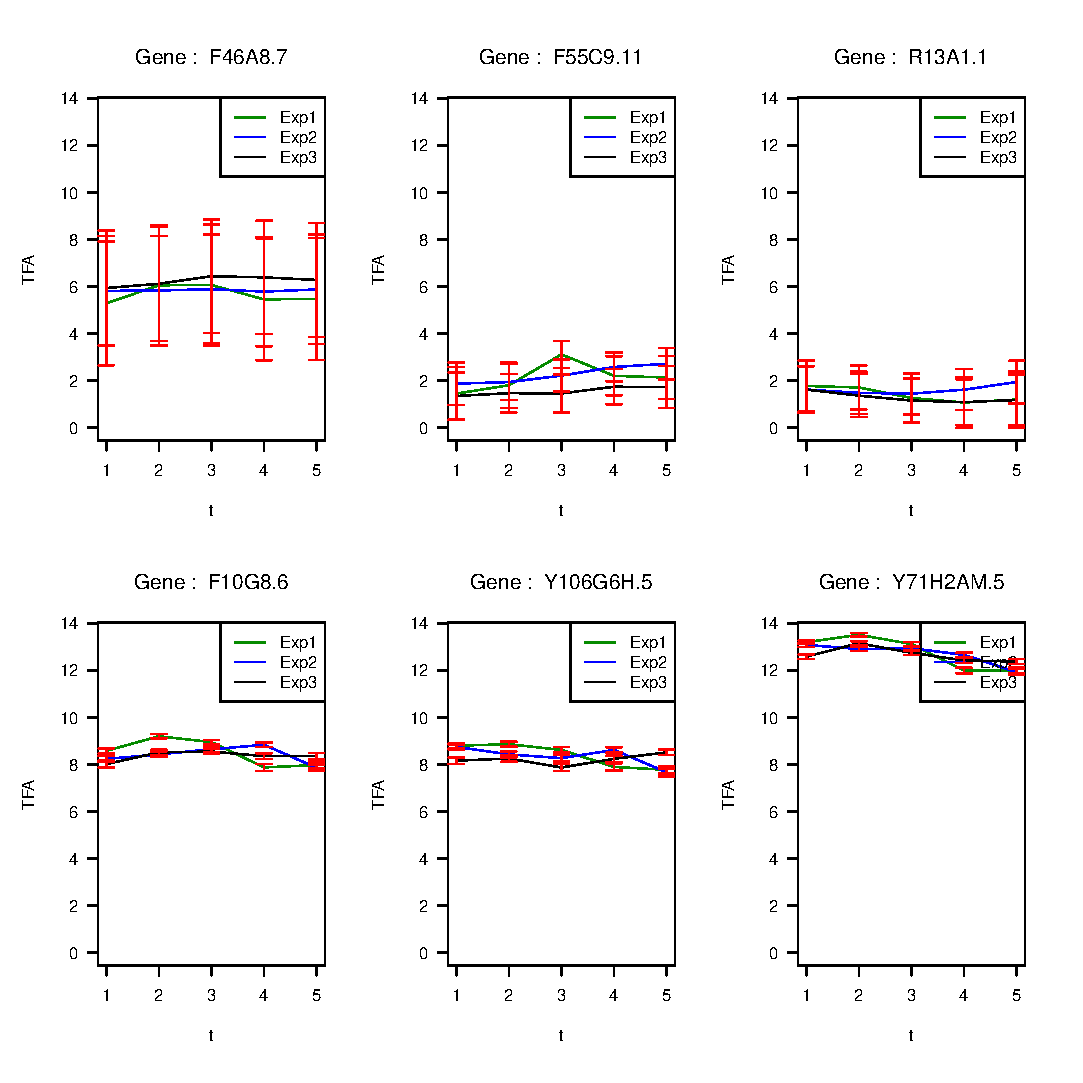
\includegraphics[width=1.0\linewidth]{picture/T20B12_8_3.eps}
      \caption{Gene Specific TFA of T20B12.8}
      \end{figure}

      %\end{block}

      
      %-- Block 3-3
      %--------------------------------------------------------------------------------------------
      %\begin{block
      Gene Specific TFA of ZK370.2
      
      \begin{figure}
      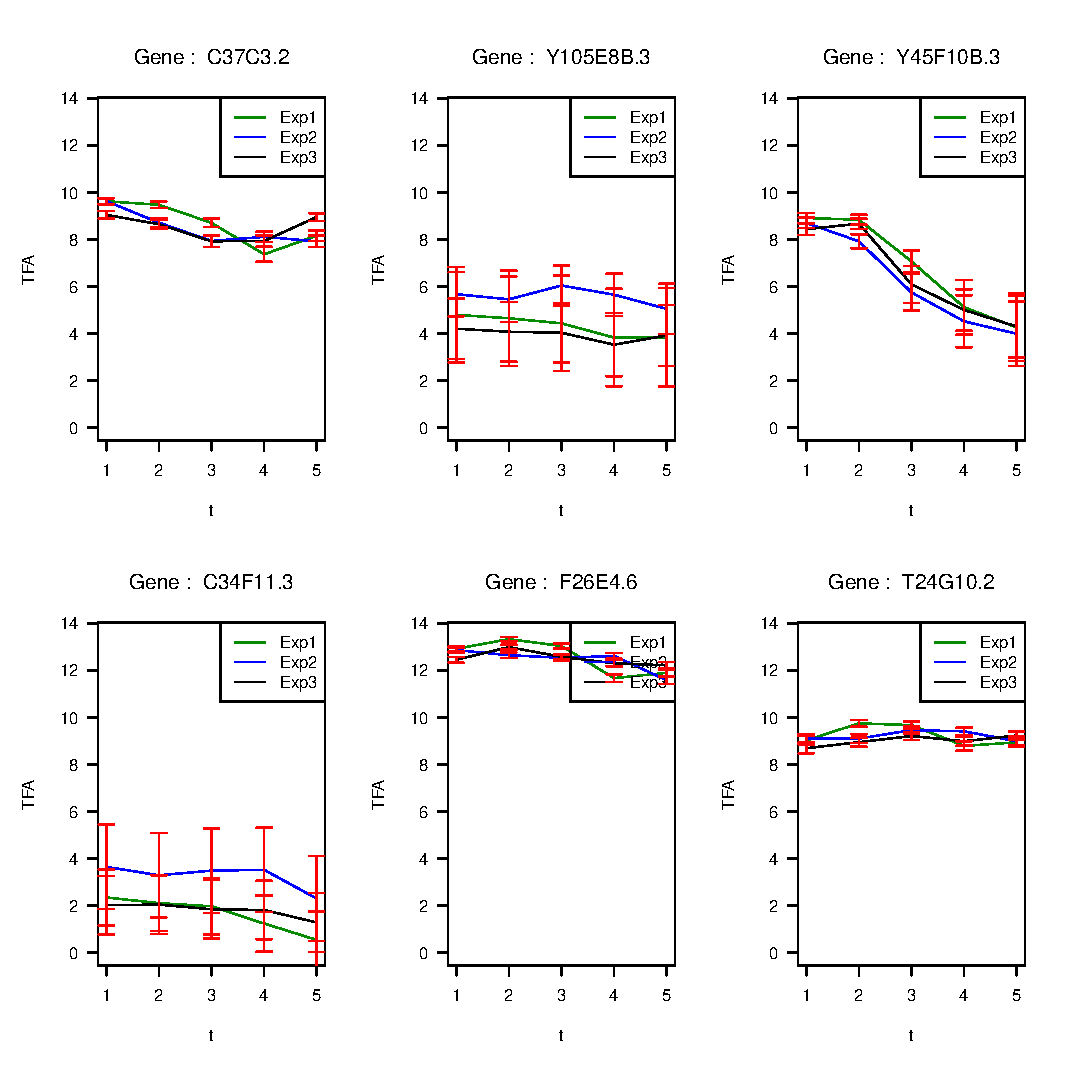
\includegraphics[width=1.0\linewidth]{picture/ZK370_2_3.eps}
      \caption{Gene Specific TFA of ZK370.2}
      \end{figure}

      %\end{block}




\section{Conclusions}\label{conclusions}
We with ~\cite{mar:01}worked hard, and achieved very little.~\cite{Arif:02}. We worked hard, and achieved very little. We worked hard, and achieved very little.

\bibliographystyle{abbrv}
\bibliography{bib_chipDyno}

\end{document}
%This is never printed
